\subsection{Problem Insights} \label{sec:insight}
Based on the observations and deep analysis, we know that there are seven page types, and the updates among them always trigger additional IOTLB flushes.
In particular, segment descriptor pages are rarely updated, as they are treated as almost const structures.
However, the page-table pages are frequently updated from/to writable pages.
These updates that are driven by the process creations and exits are frequently triggered in the whole life cycle of a running system.
Thus, they are becoming the main source for contributing the additional IOTLB flushing.

The additional IOTLB flushes are likely to let the DMA address
translations take the slow and inefficient page-table path,
instead of taking the fast and efficient IOTLB path (Figure~\ref{fig:dma-add-trans}), which inevitably lowers the
speed of the whole DMA transfering, especially for the high performance devices.


In brief, we summarize all these into three key points, which are listed as follows:
\begin{enumerate}
\item (O1) Each page-type change triggers the invalidation of at least one IOTLB entry.
\item (O2) The main source of causing IOTLB flush is the page-type changes between writable pages and page-table pages (see figure~\ref{fig:pro-ill}).
\item (O3) The additional IOTLB flushes inevitably have negative impacts on the I/O performance of the peripheral devices.
\end{enumerate}

\begin{figure}[ht]
\centering
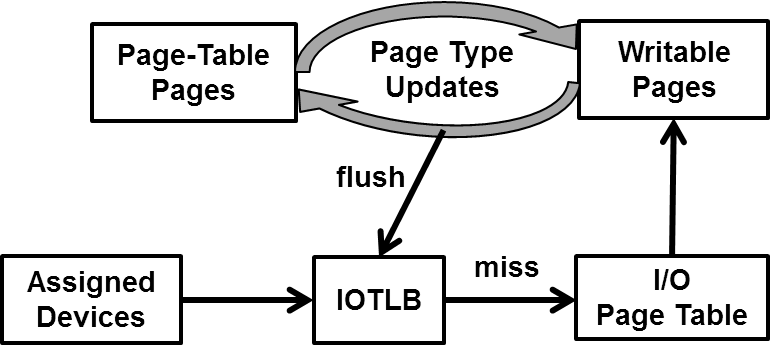
\includegraphics[width=0.5\textwidth]{image/background/problem-illustration.png} \\
\caption{Problem Illustration}
\label{fig:pro-ill}
\end{figure}

